% Please do not delete!  thanks! -- zach
% !TEX root = ../../main.tex

\begin{figure}[ht]
\label{solution:mockup_search}
\caption{Mock up of search setup screen}
\centering
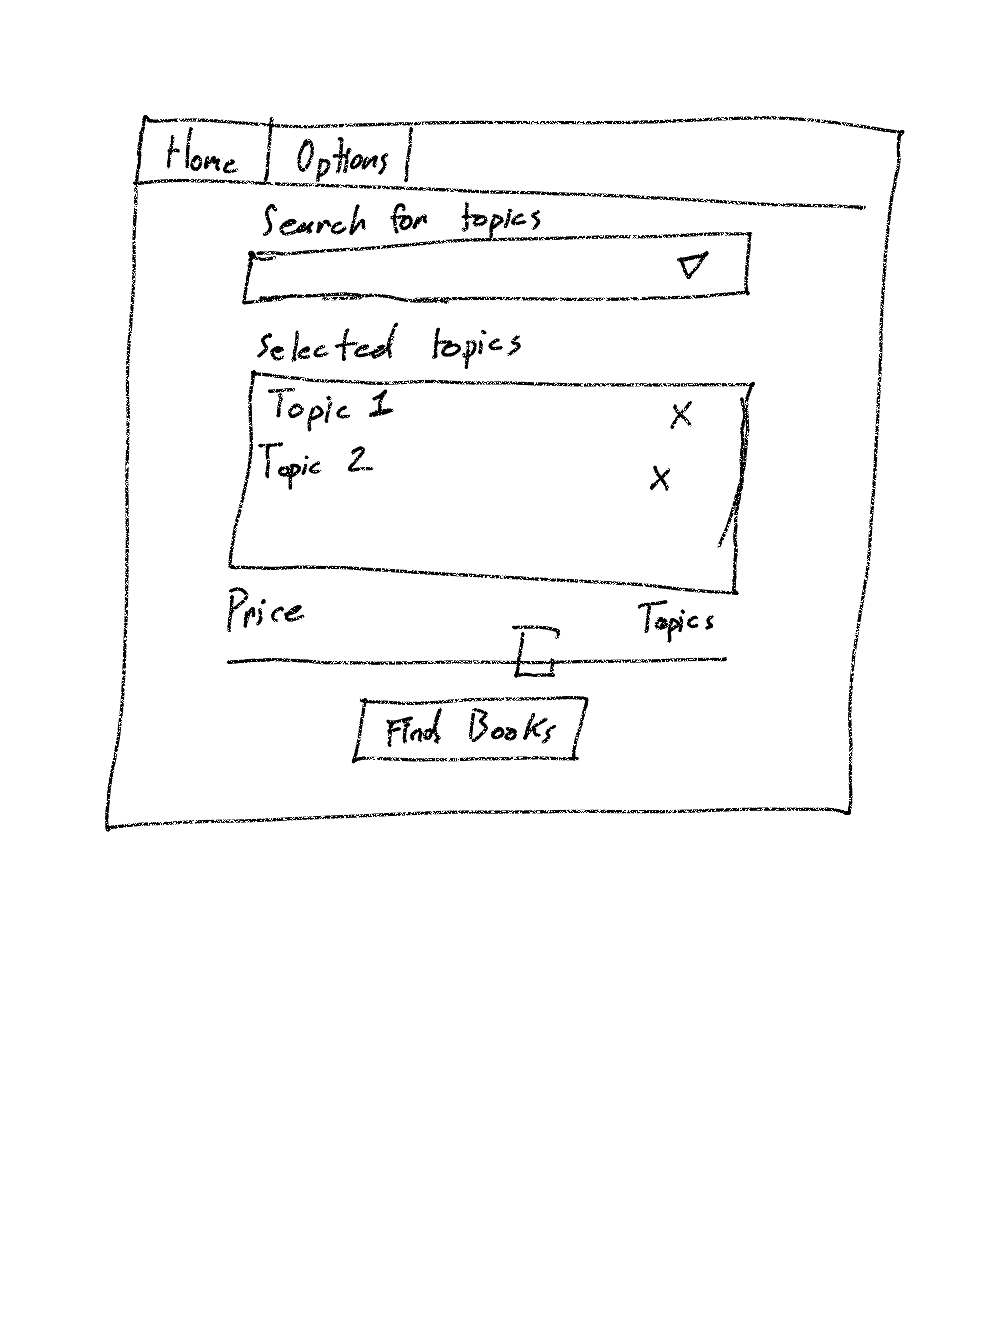
\includegraphics[width=0.5\textwidth]{search_setup}
\end{figure}

The web app is the final component of this architecture and it serves to tie the previous two components together.
The app provides the UI to the algorithms, allowing professors to log in and select a set of subjects they wish to teach on, then it should present them with a UI for searching for topics in our database.  
It should then allow them to create a list of topics to suggest books for.
Once the list has been generated, the tool should search against the book databases it has access to using the algorithms outlined in the previous sections.

\begin{figure}[ht]
\label{solution:mockup_search}
\caption{Mock up of search results screen}
\centering
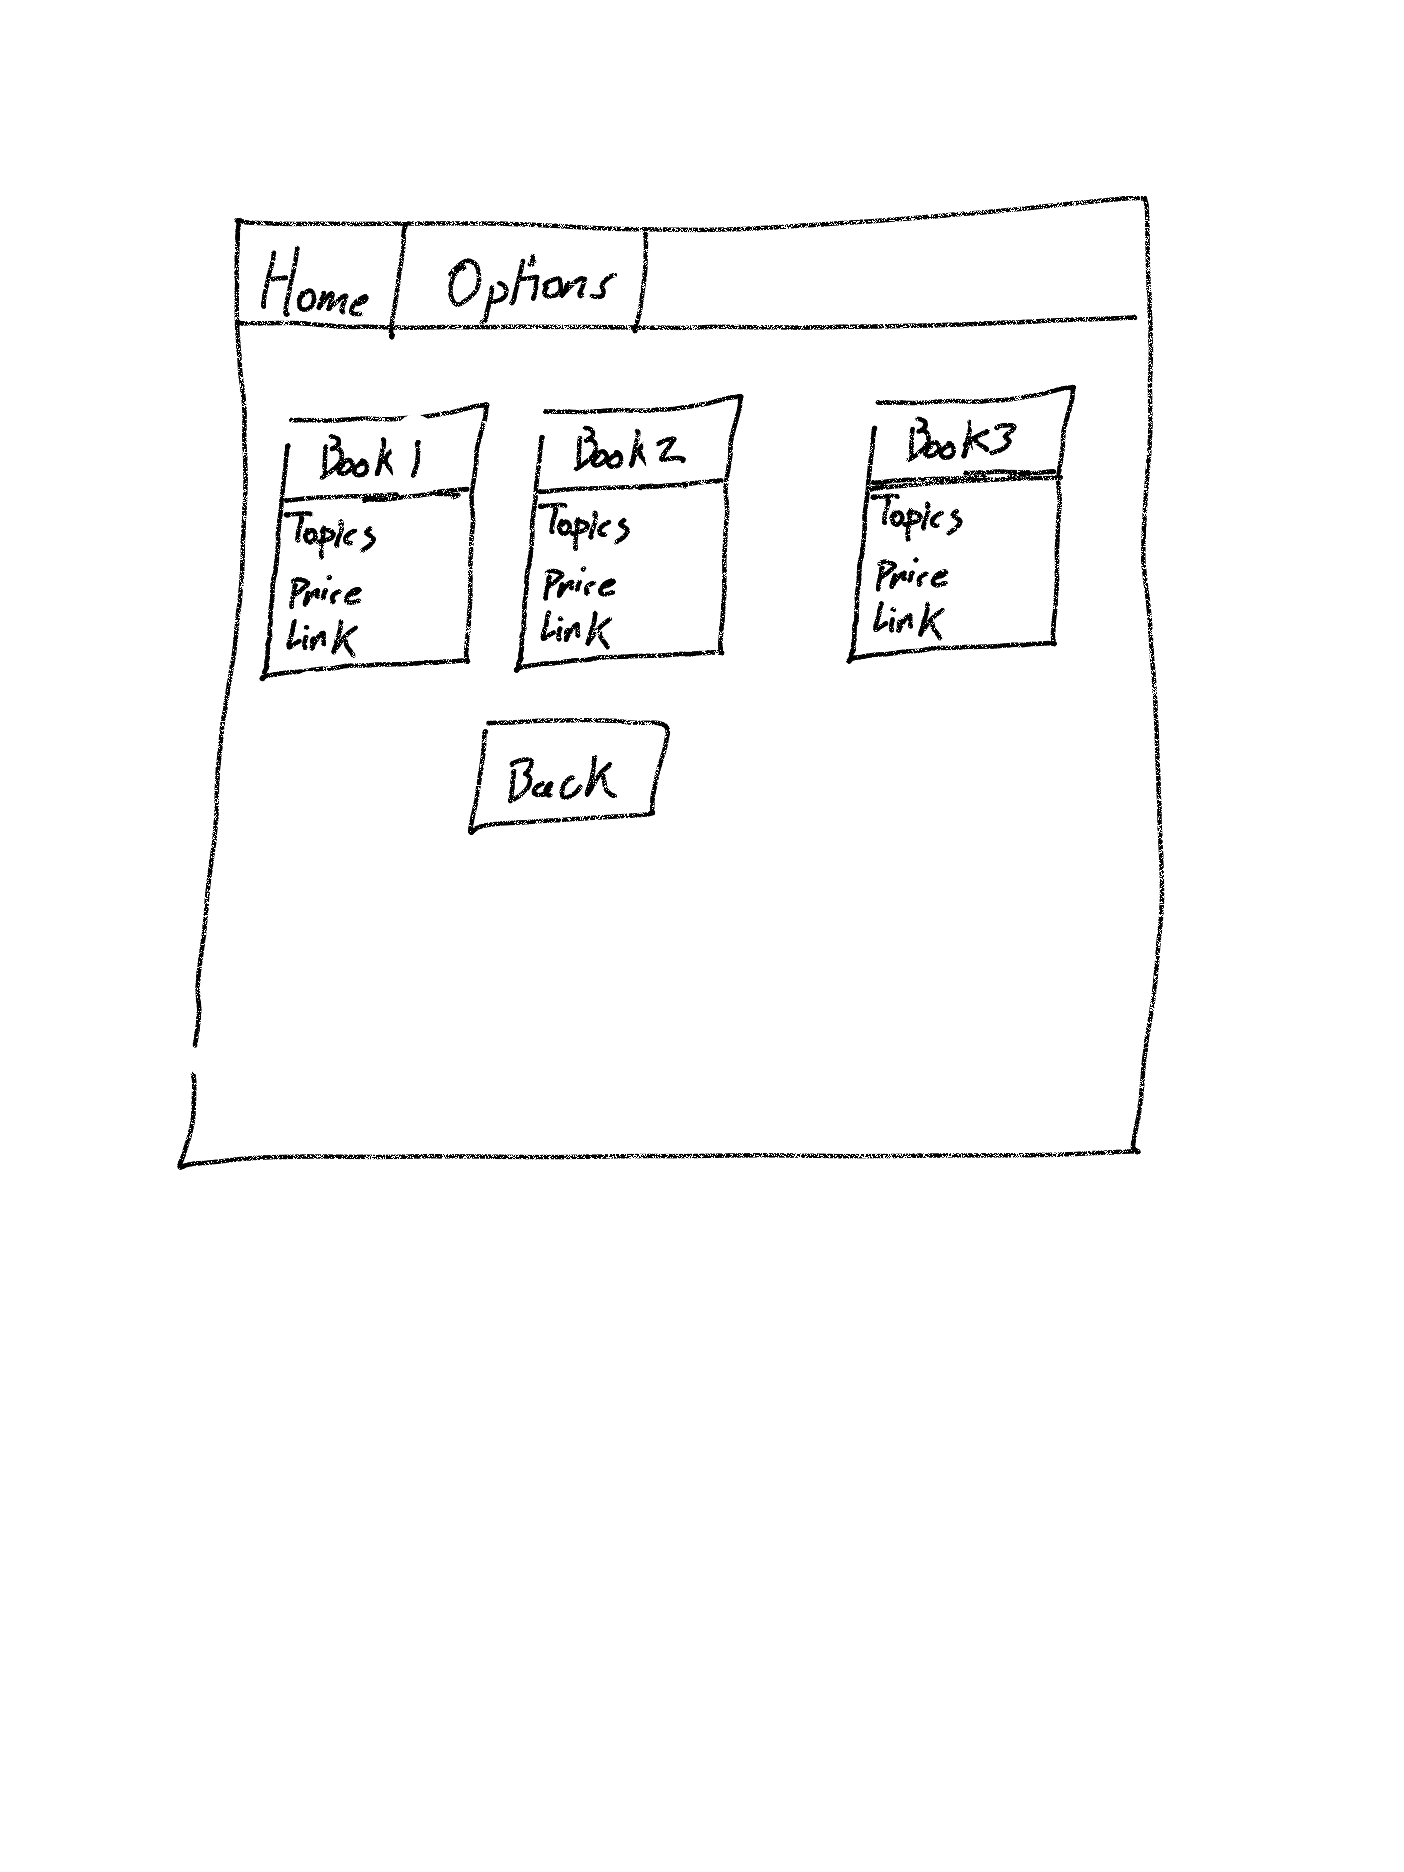
\includegraphics[width=0.5\textwidth]{search_results}
\end{figure}

We will develop this app in either the MEAN stack or some variant thereof.  (Does it make more sense to just use Django since we are writing learning algorithms in Python?)
The front-end will be developed using Bootstrap to save time in developing a useful, mobile friendly UI.
In the end, the app itself will be a single-page web app that includes minimal authentication features.  
The real complexity of this app is in the learning algorithms and the suggestion engine, so the front end of the app itself needs only to be a client to reach out to those algorithms.  